\documentclass{beamer}

\title{How to (not) Store Your Password}
\subtitle{\url{http://surl.dk/g0n/}}
\author{Ronni Elken Lindsgaard \\ rel@zx.dk \\ @rlindsgaard}
\date{2016-09-01}

\usetheme{metropolis}

\usepackage{graphicx}

\begin{document}

\begin{frame}
  \maketitle
\end{frame}

\begin{frame}
  \tableofcontents
\end{frame}

\section{Analysis}
\begin{frame}{Online password managers}
  Benefits:
  \begin{itemize}
    \item Portable
    \item Organisational sharing
    \item Not on your machine
    \item Strong passwords
  \end{itemize}
  Problems:
  \begin{itemize}
    \item Not on your machine \footnote{\url{http://www.martinvigo.com/even-the-lastpass-will-be-stolen-deal-with-it/}}
  \end{itemize}
  Attack vectors:
  \begin{itemize}
    \item Keylogging
    \item Phishing
    \item Database compromise
  \end{itemize}
\end{frame}

\begin{frame}{Offline password managers}
  Benefits:
  \begin{itemize}
    \item Stored on your machine
    \item Encrypted password storage
    \item Strong passwords
  \end{itemize}
  Problems:
  \begin{itemize}
    \item One key to the kingdom
    \item Not portable
    \item It's still stored (CVE-2015-8378)
  \end{itemize}
  Attack vectors:
  \begin{itemize}
    \item Keylogging attacks
    \item Computer/storage compromise
  \end{itemize}
\end{frame}

\begin{frame}{Let's make things better}
  \begin{itemize}
    \item Secure passwords.
    \item Domain specific passwords.
    \item Configurable.
    \item Easy to use and remember.
    \item {\color{red} No password storage!}
  \end{itemize}
\end{frame}

\section{Methodology}
\subsection{Secure Passwords}
\begin{frame}{Secure passwords}
  \begin{itemize}
    \item High entropy (e.g. NIST\footnote{\url{http://wayback.archive.org/web/20040712152833/http://csrc.nist.gov/publications/nistpubs/800-63/SP800-63v6_3_3.pdf}})
    \item Passphrases: a sentence that is not too long to remember
    \item Schneier: ASSt's!2\_2r \footnote{\url{https://www.schneier.com/blog/archives/2014/03/choosing_secure_1.html}, \url{http://robinmessage.com/2014/03/why-bruce-schneier-is-wrong-about-passwords/}}
    \item Troy Hunt: Should be too complex to remember! \footnote{\url{https://www.troyhunt.com/only-secure-password-is-one-you-cant/}}
  \end{itemize}
\end{frame}

\subsection{Generating Secure Passwords}
\begin{frame}[fragile]{Deterministic Pseudo Random Number}
  \begin{block}{Example}
    \begin{verbatim}
    % echo "naturalbornhacker" | md5sum -
    04d1530d764932ccbff01c185a283c8e  -
    \end{verbatim}
  \end{block}
\end{frame}

\begin{frame}[fragile]{Generating the password}
  \begin{verbatim}
hash = 04d1530d764932ccbff
alphabet = abcdABCD1234!"#_

password = aA"bBda"DCA2dc!!__
  \end{verbatim}
\end{frame}

\begin{frame}[fragile]{Domain specific passwords}
  \begin{verbatim}
function g(str password, str context) {
  echo hash(password + context)
}
g(naturalbornhacker, bornhack.dk)
// 1Fvcck'XE%j_cD%7oHV'A0_COrl"fK}}S,:'
g(naturalbornhacker, github.com)
// ;YR|_>(sJXgQK2S%KvSS"zH_43b6z_yN
  \end{verbatim}
\end{frame}

\begin{frame}[fragile]{Session key}
  \begin{itemize}
    \item Hash function seed
    \item Synchronously encrypt configuration
    \item Mitigate shoulder surfing
  \end{itemize}
\end{frame}

\section{Implementations}
\subsection{Related work}
\begin{frame}{PwdHash}
  \begin{itemize}
    \item \url{https://pwdhash.com/}
    \item Stanford Paper 2004 \footnote{\url{https://crypto.stanford.edu/PwdHash/}}
    \item Browser plugin
    \item Outdated security (DOM)
    \item No special characters
  \end{itemize}
\end{frame}

\begin{frame}{RndPhrase}
  \begin{itemize}
    \item \url{https://rndphrase.appspot.com/}
    \item \url{http://brinchj.blogspot.dk/2010/02/rndphrase.html}
    \item Johan Brinch 2009
    \item Small letters and numbers only
    \item Cubehash
    \item Browser plugin
  \end{itemize}
\end{frame}

\begin{frame}{One Shall Pass}
  \begin{itemize}
    \item \url{https://oneshallpass.com/}
    \item Up to date
    \item Various differences
    \item PBKDF2
  \end{itemize}
\end{frame}

\subsection{Introducing RndPhrase Improved}
\begin{frame}{Introducing RndPhrase Improved}
  \begin{itemize}
    \item 1.0.0a1
    \item PBKDF2 for hashing (WebCrypto)
    \item Configurable alphabet
    \item Character occurence constraints
    \item Configurable size
    \item Re-use credentials (versions)
  \end{itemize}
\end{frame}

\begin{frame}{User interface example}
  \begin{center}
    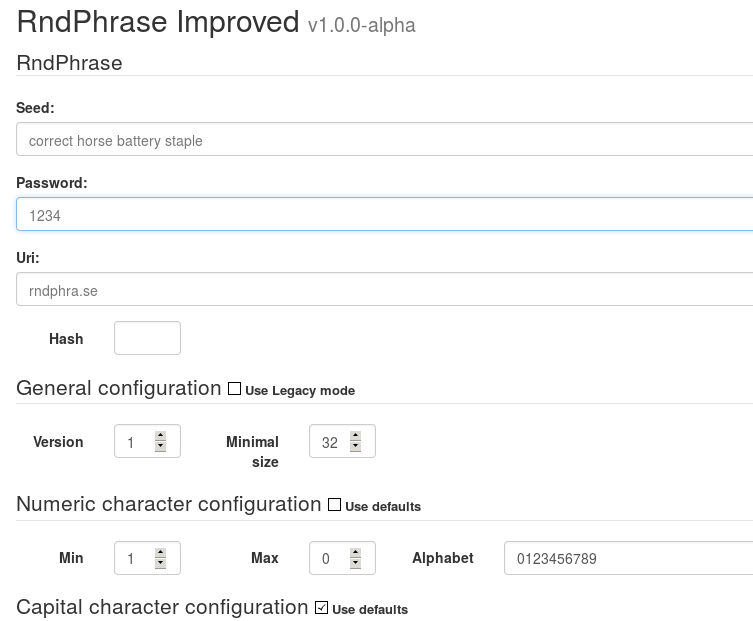
\includegraphics[scale=0.35]{rndphrase-screenshot.png}
  \end{center}
\end{frame}

\begin{frame}{Security Analysis}
  \begin{itemize}
    \item Keylogging and other active attacks still a problem
    \item No necessary storage though
  \end{itemize}
\end{frame}

\begin{frame}{Moar?}
  \begin{itemize}
    \item \url{https://rndphra.se}
    \item \url{https://github.com/RndPhrase}
    \item \url{http://rlindsgaard.github.io/2016/01/29/rndphrase-roadmap.html}
  \end{itemize}
\end{frame}
\end{document}
